\section{Take Four Problem}\label{sec:takeforproblem}
Kontrovers soll dieses Paper mit der Thematik beginnen, wann es akzeptabel ist, nicht
grundsätzlich auf Performance zu achten. Dazu soll das \emph{Take Four Problem} genauer
betrachtet werden. Was ist das \emph{Take Four Problem}? Nun das \emph{Take Four Problem} zeigt
sechs Qualitätsmerkmale an Software, die im folgenden Schaubild dargestellt werden:

\begin{figure}[h]
    \centering
    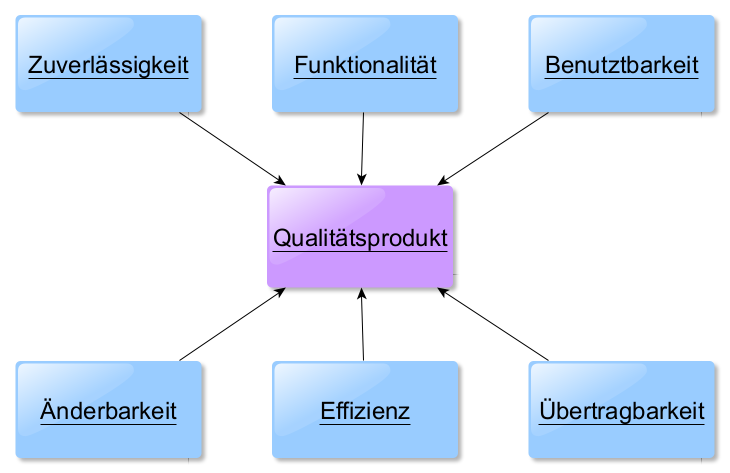
\includegraphics[width=0.5\textwidth]{bilder/ISO3}
    \caption[T4P]{Take Four Problem}
    \label{img:T4P}
\end{figure}

Das Problem, welches hier dargestellt werden soll, ist es, dass bei der Entwicklung von Software
sich auf vier der sechs Qualitätsmerkmale geeinigt werden muss, da sich manche Qualitätsmerkmale
gegenseitig ausschließen. Um ein konkretes Beispiel eines solchen Konfliktes zu nennen: Effizienz
und Zuverlässigkeit schließen sich gegenseitig aus, da Zuverlässigkeit viel auf Fehlertoleranz
baut und das Programm einfach performanter wird, wenn nicht jeder \emph{Pointer} auf \emph{null}
abgefragt wird. Auch die Wartbarkeit leidet meistens unter der Effizienz, was den Code dann schlechter zu lesen oder zu erweitern ist.
\newline
\newline
Zu sehen ist also, dass es auf den Anwendungsfall stark ankommt. Ist das Produkt eine Webseite,
die ständig weiterentwickelt wird, dann ist es viel wichtiger, dass die Software leicht
erweiterbar geschrieben ist, zumal es bei einer Webseite nicht darauf ankommt, ob sie 20 oder 200
Millisekunden braucht, um zu laden.
\newline
\newline
Andersherum gesehen ist die Performance von Echtzeit kritischen Systemen von großer Relevanz. Bei
einem Airbag beispielsweise kann es lebensentscheidend sein, ob dieser innerhalb von 20 oder 200
Millisekunden rauskommt. Im Endeffekt muss im Vorfeld entschieden werden, welche Kriterien für
die Software als wirklich relevant erachtet werden.